\documentclass[xcolor=svgnames]{beamer}
\usecolortheme[named=DarkSlateGrey]{structure}

\usepackage{braket}
\usepackage{amsmath}
\usepackage{feynmp}
\usepackage{graphicx}
\usepackage{hyperref}
\DeclareGraphicsRule{*}{mps}{*}{}
% There are many different themes available for Beamer. A comprehensive
% list with examples is given here:
% http://deic.uab.es/~iblanes/beamer_gallery/index_by_theme.html
% You can uncomment the themes below if you would like to use a different one
%\usetheme{AnnArbor}
%\usetheme{Antibes}
%\usetheme{Bergen}
%\usetheme{Berkeley}
%\usetheme{Berlin}
%\usetheme{Boadilla}
%\usetheme{boxes}
%\usetheme{CambridgeUS}
%\usetheme{Copenhagen}
%\usetheme{Darmstadt}
%\usetheme{default}
%\usetheme{Frankfurt}
%\usetheme{Goettingen}
%\usetheme{Hannover}
%\usetheme{Ilmenau}
%\usetheme{JuanLesPins}
%\usetheme{Luebeck}
%\usetheme{Madrid}
%\usetheme{Malmoe}
%\usetheme{Marburg}
%\usetheme{Montpellier}
%\usetheme{PaloAlto}
%\usetheme{Pittsburgh}
%\usetheme{Rochester}
%\usetheme{Singapore}
%\usetheme{Szeged}
\usetheme{Warsaw}
\setbeamertemplate{footline}[frame number]
\setbeamertemplate{navigation symbols}{}

\title{Scout Status Report}
% A subtitle is optional and this may be deleted
\subtitle{February 2016}

\author{Morgan Askins}
% - Give the names in the same order as the appear in the paper.
% - Use the \inst{?} command only if the authors have different
%   affiliation.

\institute[] % (optional, but mostly needed)
{
  %\inst{1}%
}
% - Use the \inst command only if there are several affiliations.
% - Keep it simple, no one is interested in your street address.

\date{\today}
% - Either use conference name or its abbreviation.
% - Not really informative to the audience, more for people (including
%   yourself) who are reading the slides online

\subject{Physics}
% This is only inserted into the PDF information catalog. Can be left
% out. 

% If you have a file called "university-logo-filename.xxx", where xxx
% is a graphic format that can be processed by latex or pdflatex,
% resp., then you can add a logo as follows:

% \pgfdeclareimage[height=0.5cm]{university-logo}{university-logo-filename}
% \logo{\pgfuseimage{university-logo}}

% Delete this, if you do not want the table of contents to pop up at
% the beginning of each subsection:
%% \AtBeginSubsection[]
%% {
%%   \begin{frame}<beamer>{Outline}
%%     \tableofcontents[currentsection,currentsubsection]
%%   \end{frame}
%% }
\AtBeginSection[]
{
  \begin{frame}<beamer>{Outline}
    \tableofcontents[currentsection]
  \end{frame}
}

\newcommand{\backupbegin}{
   \newcounter{framenumbervorappendix}
   \setcounter{framenumbervorappendix}{\value{framenumber}}
}
\newcommand{\backupend}{
   \addtocounter{framenumbervorappendix}{-\value{framenumber}}
   \addtocounter{framenumber}{\value{framenumbervorappendix}} 
}

% Let's get started
\begin{document}
% Uncomment this and the end{fmffile} for feynman diagrams
% \begin{fmffile}{feyn/quals}

{\setbeamertemplate{footline}{}
\begin{frame}[noframenumbering]
  \titlepage
\end{frame}
}

%\begin{frame}{Outline}
%  \tableofcontents
%  % You might wish to add the option [pausesections]
%\end{frame}

% Section and subsections will appear in the presentation overview
% and table of contents.

%%%%%%%%%%%%%%%%%%%%%%%%%%%%%%%%%%%%%
%\section{First Section}
%\subsection{First Subsection}
%\begin{frame}[]{}
%  \begin{columns}
%    \begin{column}{0.5\textwidth}
%      \begin{itemize}
%        \item a
%        \item b
%        \item c
%      \end{itemize}
%    \end{column}
%    \begin{column}{0.5\textwidth}
%      \begin{enumerate}
%        \item one
%        \item two
%        \item three
%      \end{enumerate}
%    \end{column}
%  \end{columns}
%\end{frame}

\begin{frame}{Optical Coupling}
  \begin{itemize}
    \item Found two companies that produce optical gel pads, which are reusable.
    \item Flashpointcrystals: Pads are \$50 each, but 3 inch is a custom size requiring an extra \$450 to make a mold for it
    \item Saint-Gobain ... No response from customer servce
  \end{itemize}
\end{frame}

\begin{frame}{Design}
  \begin{center}
    \href{https://github.com/MorganAskins/scout/blob/master/scout.avi?raw=true}{ScoutVideo.avi}\\
    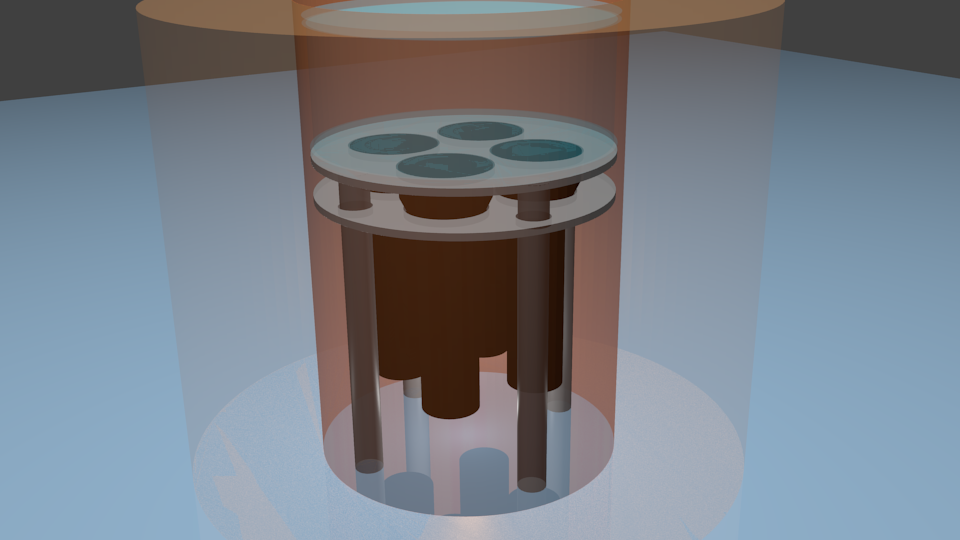
\includegraphics[width=0.5\textwidth]{../../../images/scout_render.png}
  \end{center}
\end{frame}

% \begin{frame}[t, label=bbrate]{$0\nu\beta\beta$ Rates}
%   \centering
%   \only<1>{$\boldsymbol{[T_{1/2}^{0\nu}]^{-1}}=G^{0\nu}
%     |M^{0\nu}|^2|\braket{m_\nu}|^2/m_e^2$}
%   \only<2>{$[T_{1/2}^{0\nu}]^{-1}=\boldsymbol{G^{0\nu}}
%     |M^{0\nu}|^2|\braket{m_\nu}|^2/m_e^2$}
%   \only<3>{$[T_{1/2}^{0\nu}]^{-1}=G^{0\nu}\boldsymbol{|M^{0\nu}|^2}
%     |\braket{m_\nu}|^2/m_e^2$}
%   \only<4>{$[T_{1/2}^{0\nu}]^{-1}=G^{0\nu}|M^{0\nu}|^2
%     \boldsymbol{|\braket{m_\nu}|^2}/m_e^2$}
%   \begin{columns}[t]
%     \begin{column}{0.6\textwidth}
%       \begin{itemize}
%         \only<1>{\item \textbf{$T_{1/2}^{0\nu}$: Decay half life}}
%         \only<2->{\item $T_{1/2}^{0\nu}$: Decay half life}
%         \only<2>{\item \textbf{$G^{0\nu}$: \hyperlink{phase_sup}{Phase space integral}}}
%         \only<1,3->{\item $G^{0\nu}$: Phase space integral}
%         \only<3>{\item \textbf{$|M^{0\nu}|^2$: Nuclear Matrix Element}}
%         \only<1-2,4->{\item $|M^{0\nu}|^2$: Nuclear Matrix Element}
%         \only<4>{\item \textbf{$\braket{m_\nu}$: Effective Majorana Mass}}
%         \only<1-3>{\item $\braket{m_\nu}$: Effective Majorana Mass}
%       \end{itemize}
%     \end{column}
%     \begin{column}{0.4\textwidth}
%       \only<1>{
%         \begin{itemize}
%           \item Quadratic sensitivity to Matrix element and $\nu$ mass
%           \item Very large suppression for light neutrino
%         \end{itemize}
%       }
%       \only<2>{
%         \begin{itemize}
%           \item Integral over phase space of electron E, p including coloumb effects
%           \item Numerically calculated, well understood, and agreed upon
%         \end{itemize}
%       }
%       \only<3>{
%         \begin{itemize}
%         \item Can only be determined by theoretical calculation
%         \item Random Phase Approximation, Shell Model, N-Body
%         \end{itemize}
%       }
%       \only<4>{
%         \begin{align*}
%         \braket{m_\nu} &=\sum U_{ei}^2m_i\\
%         U_{e1}^2 &=\cos^2\theta_{13}\cos^2\theta_{12}e^{i\lambda_1}\\
%         U_{e2}^2 &=\cos^2\theta_{13}\sin^2\theta_{12}e^{i\lambda_2}\\
%         U_{e3}^2 &=\sin^2\theta_{13}
%         \end{align*}
%         where $U_{ei}$ are elements of the PMNS matrix
%         \hyperlink{bbrate_mass_sup}{$\ket{\nu_l}=U^*_{lm}\ket{\nu_m}$}
%       }
%     \end{column}
%   \end{columns}
% \end{frame}


%%%%%%%%%%%%%%%%%%%%%%%%
%% BACKUP SLIDES
%%%%%%%%%%%%%%%%%%%%%%%%
%\backupbegin
%\begin{frame}{Backup}{Slides}
%\end{frame}
%\backupend
%\end{fmffile}
\end{document}
